\newpage
\appendix

\section{Visualisation of cleaned vs raw dataset}

\begin{figure}[!h]
    \centering
    \includegraphics[width = 0.8\linewidth]{"../../R/figures/raw-vs-cleaned-glob.png"}
    \caption{\label{fig:raw_vs_cleaned_glob} Visualisation of the cleaned dataset for \gls{harm} in comparison to the total raw dataset. The red and green boxes show the used extents for Europe and the native range respectively, red and green points show the cleaned presence points in their respective extents, while blue points show all points of the raw dataset.}
\end{figure}



\section{Niche analysis}

\begin{figure}[!h]
    \centering
    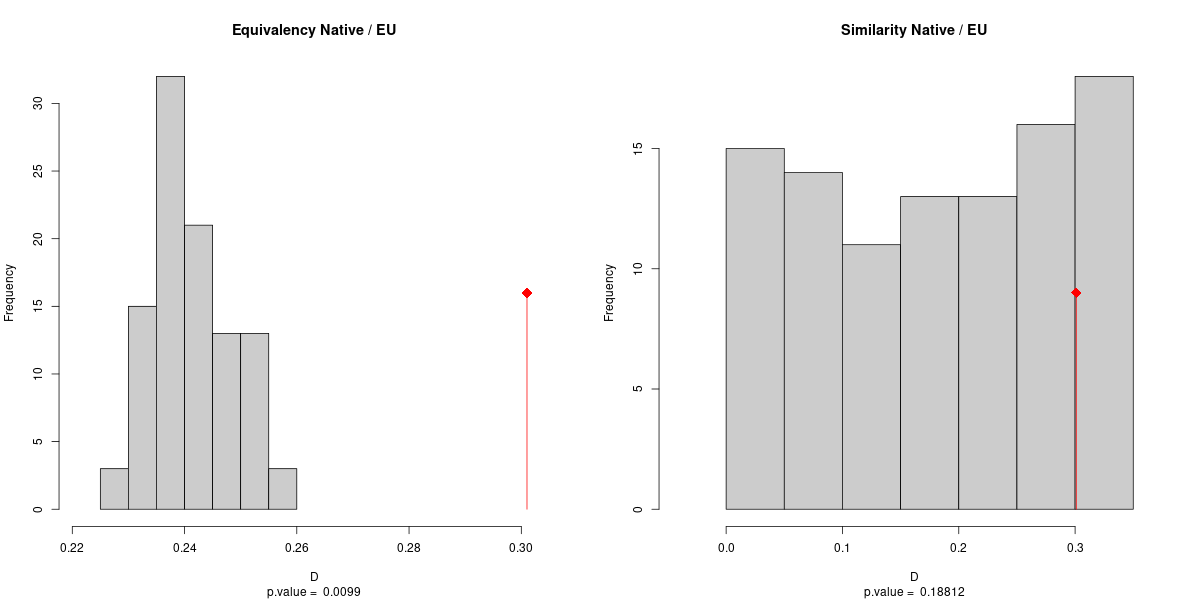
\includegraphics[width = 0.9\linewidth]{"../../R/figures/as-eu-tot-eq-sim.png"}
    \caption{\label{fig:as_eu_eq_sim} Results of the niche equivalency (left) and niche similarity (right) test comparing the native and invaded niche of \gls{harm}. Histograms of the simulated niche overlaps, the observed overlap shown as a red bar with a diamond.}
\end{figure}

\begin{figure}[!h]
    \centering
    \includegraphics[width = 0.68\linewidth]{"../../R/figures/as-eu-pca.png"}
    \caption{\label{fig:as_eu_niche_pca} Component contributions for the PCA used to conduct the niche analyses comparing the total native and invaded niches. For detail on the bioclim variables, see (Supplementary Tab. \ref{tab:bioclim}).}
\end{figure}

\begin{figure}[!h]
    \centering
    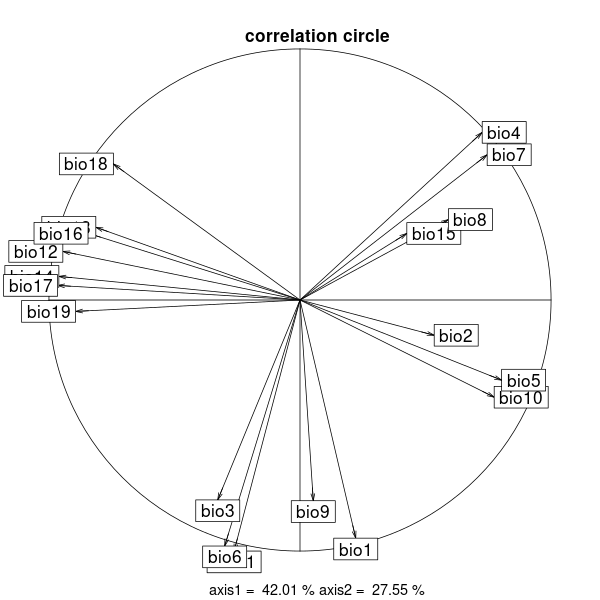
\includegraphics[width = 0.68\linewidth]{"../../R/figures/eu-years-pca.png"}
    \caption{\label{fig:eu_years_pca} Component contributions for the PCA used to conduct the niche analyses comparing each year of the invaded niche to its  following year. For detail on the bioclim variables, see (Supplementary Tab. \ref{tab:bioclim}).}
\end{figure}

\clearpage
\begin{table}[!h]
    \centering
    \caption{\label{tab:bioclim} Explanation of the bioclim variables (from CHELSA 2.x technical specifications).}
    \begin{tabular}{l l}
        \textbf{Variable} & \textbf{Explanation}
        \csvreader[head to column names]{tab-CHELSA-bioclim-expl.csv}{}{
        \\ \shortname & \longname
        }
    \end{tabular}
\end{table}


\clearpage
\section{Species distribution modelling}

\begin{table}[!h]
    \centering
    \caption{\label{tab:lc_contrib} Table showing PCA contributions for each Copernicus land cover class, Copernicus land cover class explanation in (Supplementary Tab. \ref{tab:Cop_lcc}).}
    \centerline{
        \begin{tabular}{r r*{7}{S[table-format = 1.2e2, table-align-text-pre = false, table-space-text-pre = lc]}}
            \csvreader[no head, column count = 8, late after line = \\]{tab-lc-contrib.csv}{}{\csvlinetotablerow}
        \end{tabular}
    }
\end{table}

\begin{table}[!h]
    \centering
    \caption{\label{tab:Cop_lcc} Explanation of the Copernicus land cover classes (from dataset legend).}
    \begin{tabular}{r l}
        \csvreader[no head, column count = 2, late after line = \\]{tab-Cop-lcc.csv}{}{\csvlinetotablerow}
    \end{tabular}
\end{table}

\clearpage
\begin{table}[!h]
    \centering
    \caption{\label{tab:mod_ths} Thresholds used to predict the models for the given years (inv = invaded range model (of the previous year), nat = native range model).}
    \centerline{
        \begin{tabular}{r*{11}{c}}
            \csvreader[no head, column count = 11, late after line = \\]{tab-mod-ths.csv}{}{\csvlinetotablerow}
        \end{tabular}
    }
\end{table}

\clearpage
\section{Model predictions}
\begin{figure}[!h]
    \caption{\label{fig:all_mod_preds} Predictions of each invaded range ensemble model for the year 2022, points in black showing the occurrences of the respective year, so i.e. in 2003 model it shows the occurrences of 2003, but the suitability prediction for 2022.}
    \centerline{
        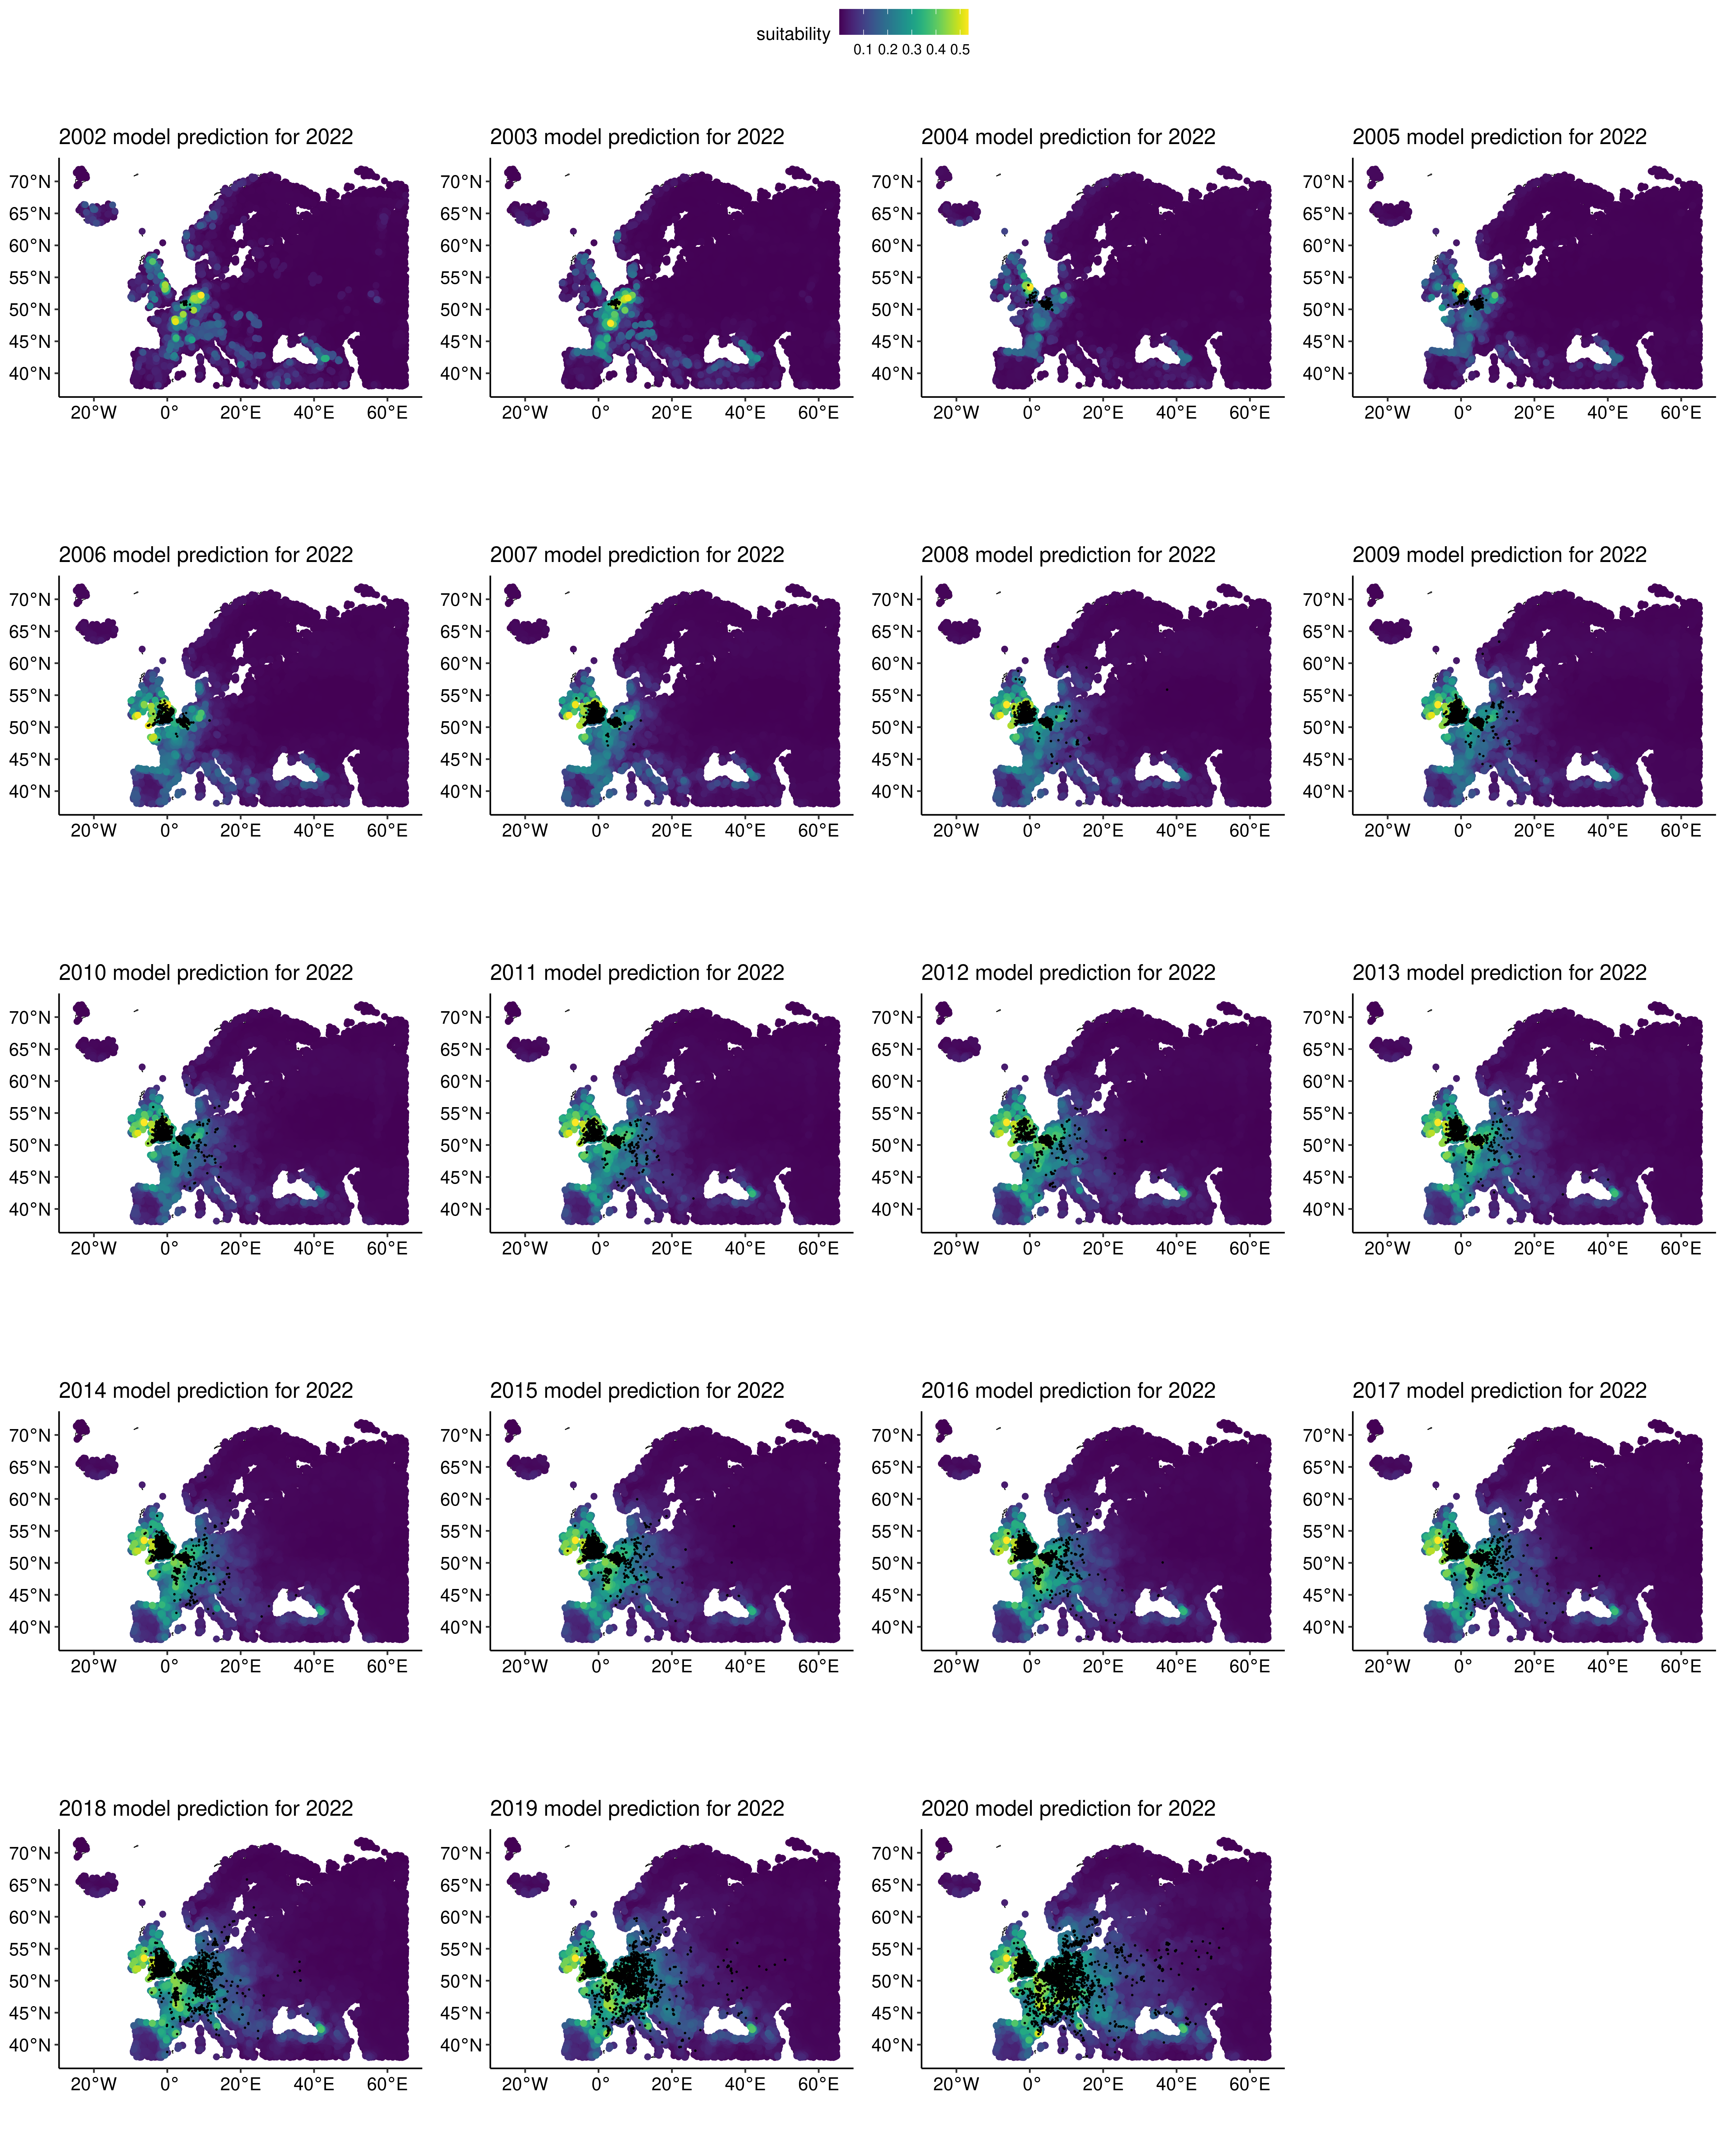
\includegraphics[width = 0.85\paperwidth, height = 0.62\paperheight]{"../../R/figures/2003to2021-mod-pred.png"}
    }
\end{figure}

\section{Model response curves} \label{sec:response_curves}

\begin{figure}[!ht]
    \caption*{Native model response curves}
    \centerline{
        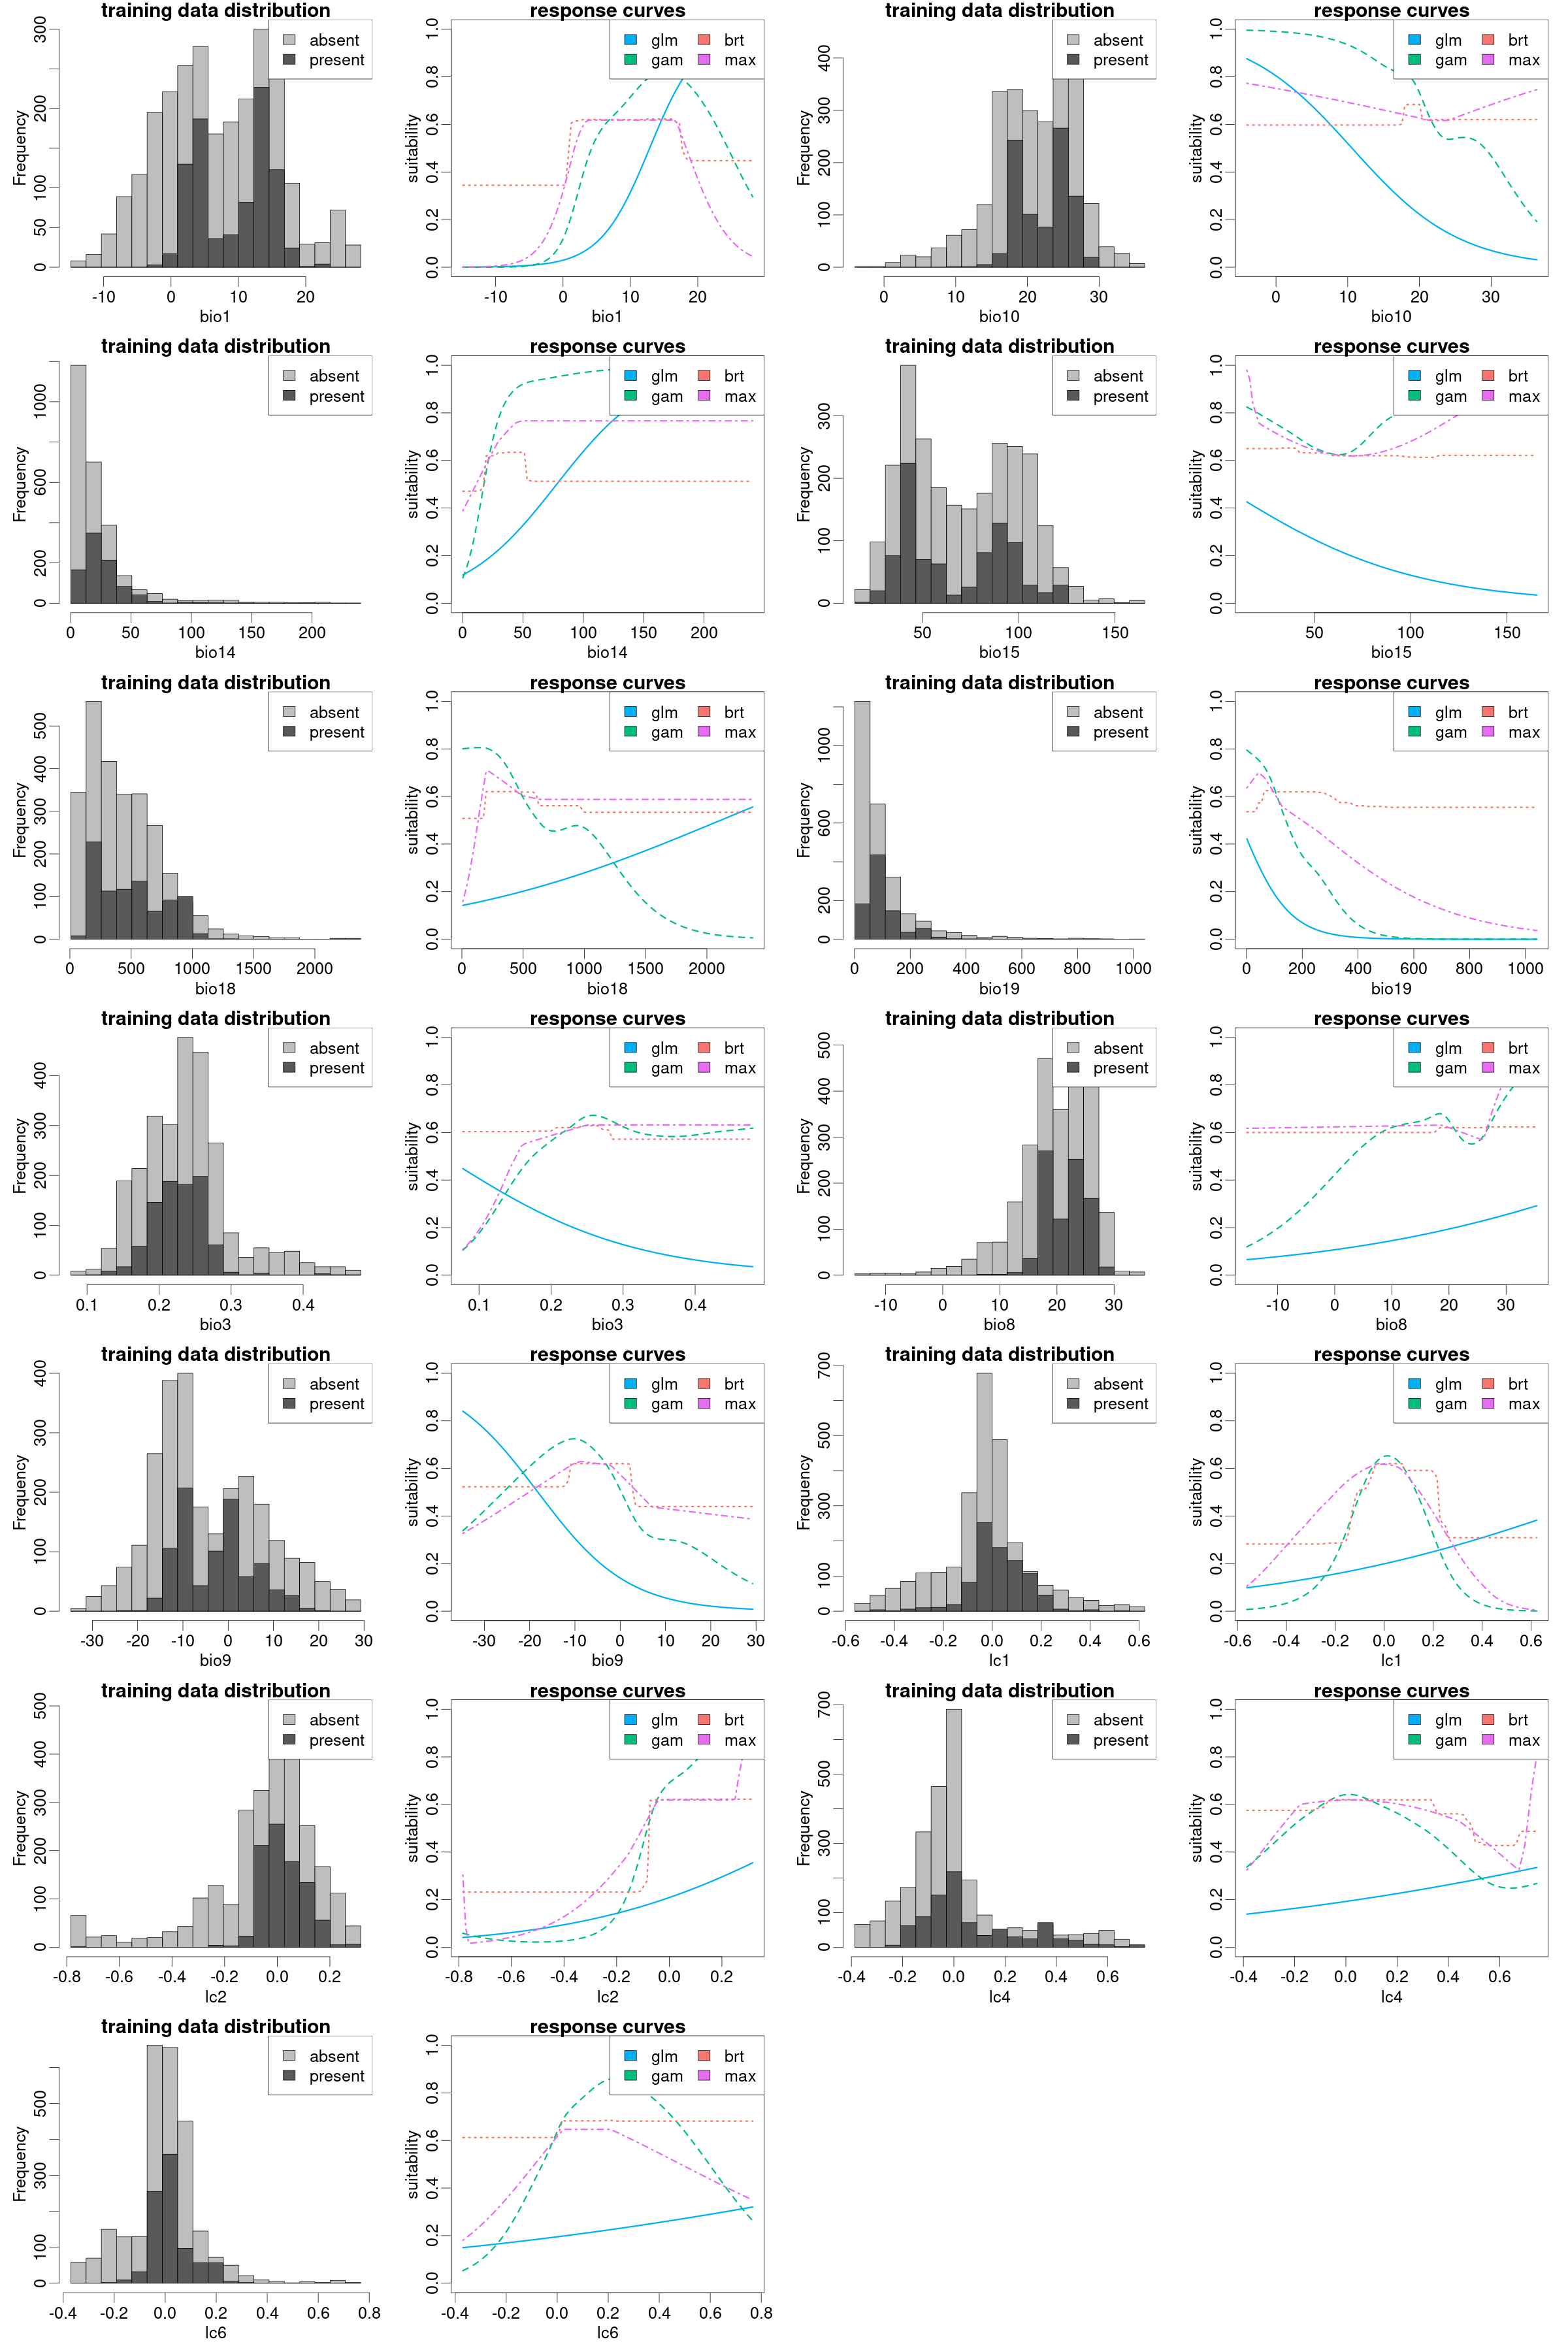
\includegraphics[width = 0.9\paperwidth, height = 0.83\paperheight]{"../../R/plots/response_curves/native_mod_resp.png"}
    }
\end{figure}

\foreach \y in {2002,...,2020}{
        \begin{figure}[!ht]
            \caption*{\y \ model response curves}
            \centerline{
                \includegraphics[width = 0.9\paperwidth, height = 0.83\paperheight]{"../../R/plots/response_curves/\y_mod_resp.png"}
            }
        \end{figure}
    }